\documentclass{beamer}

\usepackage{lmodern}
\usepackage[utf8]{inputenc}
\usepackage[T1]{fontenc}
\usepackage[style=ieee,dashed=false,backend=biber,bibencoding=utf8]{biblatex}
\usepackage{xcolor}
\usepackage{minted}
\usepackage{listings}
\usepackage{graphicx}
\usepackage{grffile}
\usepackage{hyperref}
\usepackage[ngerman]{babel}
\usepackage{csquotes}
\usepackage{caption}
\usepackage{subcaption}
\usepackage{amssymb}
\usepackage{amsmath}
\usepackage{tikz}
\usepackage{pgfplots}


\addbibresource{references/images.bib}
\addbibresource{references/scientific.bib}

\renewcommand{\lstlistlistingname}{Quellcodeverzeichnis}
\renewcommand{\lstlistingname}{Code}


\definecolor{danger}{RGB}{220, 53, 69}
\newenvironment{longlisting}{\captionsetup{type=listing}}{}

\usetheme[progressbar=frametitle]{metropolis}


\definecolor{HTWGreen}{HTML}{76B900}
\definecolor{HTWBlue}{HTML}{0082D1}
\definecolor{HTWOrange}{HTML}{FF5F00}
\definecolor{HTWGrey}{HTML}{AFAFAF}
\definecolor{HTWWhite}{HTML}{FFFFFF}
\definecolor{HTWBlack}{HTML}{000000}

\setbeamercolor{frametitle}{%
    bg=HTWGreen
}

\setbeamercolor{alerted text}{%
    fg=HTWGrey
}

\setbeamercolor{normal text}{%
    fg=HTWBlack,
    bg=HTWWhite
}

\setminted[cpp]{,
    fontsize=\footnotesize,
    linenos,
    breaklines
}


\setbeamertemplate{bibliography item}[text]
\setbeamertemplate{section in toc}[sections numbered]
\setbeamertemplate{subsection in toc}[subsections numbered]

\definecolor{htwgruen}{RGB}{118, 185, 0}
\definecolor{htwblau}{RGB}{0, 130, 209}
\definecolor{htworange}{RGB}{255, 95, 0}
\definecolor{htwgrau}{RGB}{175, 175, 175}


\newcommand*{\examiner}[1]{\gdef\insertexaminer{#1}}
\newcommand*{\matrikelNo}[1]{\gdef\insertmatrikelno{#1}}


\def\changemargin#1#2{\list{}{\rightmargin#2\leftmargin#1}\item[]}
\let\endchangemargin=\endlist

\setbeamertemplate{title page}{
    \begin{minipage}[c][\paperheight]{\textwidth}
        \ifx\inserttitlegraphic\@empty\else\usebeamertemplate*{title graphic}\fi
        \vfill
        \vfill
        \ifx\inserttitle\@empty\else\usebeamertemplate*{title}\fi
        \ifx\insertsubtitle\@empty\else\usebeamertemplate*{subtitle}\fi
        \usebeamertemplate*{title separator}
        \vspace*{1.2em}
        \begin{minipage}[t]{.5\textwidth}
            \ifx\insertauthor\@empty\else
            \textbf{Autor:} \par
            \small{\insertauthor} \par
            \ifx\insertmatrikelno\@empty\else \small{\insertmatrikelno} \par \fi
            \fi
            \ifx\insertinstitute\@empty\else \small{\insertinstitute} \par \fi

        \end{minipage}
        \begin{minipage}[t]{.5\textwidth}
            \ifx\insertexaminer\@empty\else \textbf{Betreuer:} \par \small{\insertexaminer} \par \fi
        \end{minipage}
        
        \vspace*{3.2em}
        \ifx\insertdate\@empty\else \tiny{\insertdate} \par \fi

        \vfill
        \vspace*{1mm}
    \end{minipage}
}

\title{Das rkmh toolkit und seine Einsatzgebiete}
\subtitle{Seminar zu aktuellen Entwicklungen}
\author{Christoph Stach}
\titlegraphic{
\includegraphics[width=0.25\textwidth]{images/Q04_HTW_Berlin_Logo_quer_pos_FARBIG_RGB.jpg}}
\examiner{Prof. Dr.-Ing. Dabrowski}
\matrikelNo{555912}

\date{\today}
\institute{HTW Berlin}


\begin{document}

\maketitle

\begin{frame}{Inhalt}
    \tableofcontents
\end{frame}
\section{Einleitung}

\begin{frame}{Einleitung}
    \begin{itemize}
        \item DNA: (A)denin, (T)hymin, (G)uanin und (C)ytosin \pause
        \item Proben können sequenziert \pause
        \item Reads aus Tesdaten haben eine Länge von \textasciitilde 250 Proteien-Basenpaaren \pause
        \item Datensätze: FASTQ, FASTA
    \end{itemize}
\end{frame}


\begin{frame}[fragile]{Einleitung - FASTA Beispiel\footnote{\url{http://www.cbs.dtu.dk/services/NetGene2/fasta.php}}}
    \begin{minted}{text}
>HSBGPG Human gene for bone gla protein (BGP)
GGCAGATTCCCCCTAGACCCGCCCGCACCATGGTCAGGCATGCCCCTCCTCATCGCTGGGCACAGCCCAGAGGGT
ATAAACAGTGCTGGAGGCTGGCGGGGCAGGCCAGCTGAGTCCTGAGCAGCAGCCCAGCGCAGCCACCGAGACACC
ATGAGAGCCCTCACACTCCTCGCCCTATTGGCCCTGGCCGCACTTTGCATCGCTGGCCAGGCAGGTGAGTGCCCC
CACCTCCCCTCAGGCCGCATTGCAGTGGGGGCTGAGAGGAGGAAGCACCATGGCCCACCTCTTCTCACCCCTTTG
GCTGGCAGTCCCTTTGCAGTCTAACCACCTTGTTGCAGGCTCAATCCATTTGCCCCAGCTCTGCCCTTGCAGAGG
GAGAGGAGGGAAGAGCAAGCTGCCCGAGACGCAGGGGAAGGAGGATGAGGGCCCTGGGGATGAGCTGGGGTGAAC
CAGGCTCCCTTTCCTTTGCAGGTGCGAAGCCCAGCGGTGCAGAGTCCAGCAAAGGTGCAGGTATGAGGATGGACC
TGATGGGTTCCTGGACCCTCCCCTCTCACCCTGGTCCCTCAGTCTCATTCCCCCACTCCTGCCACCTCCTGTCTG
GCCATCAGGAAGGCCAGCCTGCTCCCCACCTGATCCTCCCAAACCCAGAGCCACCTGATGCCTGCCCCTCTGCTC
CACAGCCTTTGTGTCCAAGCAGGAGGGCAGCGAGGTAGTGAAGAGACCCAGGCGCTACCTGTATCAATGGCTGGG
GTGAGAGAAAAGGCAGAGCTGGGCCAAGGCCCTGCCTCTCCGGGATGGTCTGTGGGGGAGCTGCAGCAGGGAGTG
GCCTCTCTGGGTTGTGGTGGGGGTACAGGCAGCCTGCCCTGGTGGGCACCCTGGAGCCCCATGTGTAGGGAGAGG
AGGGATGGGCATTTTGCACGGGGGCTGATGCCACCACGTCGGGTGTCTCAGAGCCCCAGTCCCCTACCCGGATCC
CCTGGAGCCCAGGAGGGAGGTGTGTGAGCTCAATCCGGACTGTGACGAGTTGGCTGACCACATCGGCTTTCAGGA
GGCCTATCGGCGCTTCTACGGCCCGGTCTAGGGTGTCGCTCTGCTGGCCTGGCCGGCAACCCCAGTTCTGCTCCT
CTCCAGGCACCCTTCTTTCCTCTTCCCCTTGCCCTTGCCCTGACCTCCCAGCCCTATGGATGTGGGGTCCCCATC
ATCCCAGCTGCTCCCAAATAAACTCCAGAAG
    \end{minted}
\end{frame}

\begin{frame}[fragile]{Einleitung - FASTQ Beispiel\footnote{\url{https://github.com/edawson/rkmh_sim_data}}}
    \begin{minted}{text}
631232382/31100220/2202403222222222223125251225244225125230222124223302
@HPV16|Z109|B2_601_1122_0_1_0_0_15:1:0_11:0:0_71933/2
CCCCCACTTCCACCACTTATACTGCTACATGGTGTTTCAGTCTCATGGCGCCCTTCTACCTGTAACGATTC
+
236520202/2132221222221541022222022222323023213421222445242222/12250234
@HPV16|Z109|B2_388_953_0_1_0_0_10:0:0_11:0:0_e0828/2
ATCTACGGACTAATATTATTGTCTACACATCCACTAATATCACTCAAGTGGACTACCCAAATACTTTCGTT
+
3232112242221235221/3321543020232443253222/3122203042202032425044/07245
@HPV16|Z109|B2_4780_4199_1_0_0_0_11:0:0_3:1:0_ba60c/2
TTTATTGTTTGTTTTGTTTGTTTTTTAAATAAACTGTTATTACTTAACAATGCGACACAAACGTTCTGCAA
+
221122234222229205202222232221262370322524352255/3212123232303234422330
@HPV16|Z109|B2_5953_6522_0_1_0_0_13:0:0_11:1:0_cc11b/1
GTGTAGGTGTTGAGGTAGGTCGCGGTCAGCCATTAGGTGTGGGCATTAGTGGCCATCCTTTATTAAATAAA
    \end{minted}
\end{frame}

\section{Rkmh}

\begin{frame}{Rkmh I}
    \begin{itemize}
        \item \textbf{Viral coinfection analysis using a MinHash toolkit \cite{rkmh}} \pause
        \item Human papillomavirus (HPV) \pause
        \item HPV hat viele unterschiedliche Typen bzw. Abstammungslinien \pause
        \item Co-Infektionen verschiedener Abstammungslinien sind üblich \pause
        \item Davon sind nur einige hoch krebserzeugend
    \end{itemize}
\end{frame}

\begin{frame}{Rkmh II}
    \begin{itemize}
        \item rkmh klassifiziert Reads aus FASTQ-Dateien \pause
        \item Jeder Read wird mit einer Menge von Referenzgenomen verglichen \pause
        \item rkmh weist jedem Read das Referenzgenom zu mit dem es die höchste Übereinstimmung hat \pause
        \item Für den Vergleich bedient sich rkmh der MinHash-Methode  aus dem Bereich der Textanalyse \pause
        \item \textbf{On the Resemblance and Containment of Documents \cite{minhash}}
    \end{itemize}
\end{frame}
\section{Shingling}

\begin{frame}{Shingling I}
    \begin{itemize}
        \item n-grams, k-mers, k-shingles \pause
        \item Sequenzen aus Wörtern oder Buchstaben werden geshingelt \pause
        \item Durch Shingling entsteht eine Menge von Shinglen ohne doppelte Vorkommen \pause
        \item Geshingelte Sequenzen können besser mit einander verglichen werden
    \end{itemize}
\end{frame}


\begin{frame}{Shingling II - Beispiel}
    Gegeben sind zwei Dokumente $ A = ``ATGGTAT" $ und $ B = ``TGGCAGT" $ und eine Shinglelänge von $ k = 3 $. \pause
    
    \begin{example}
        \begin{equation*}
            \begin{split}
                S_3(A) = \{ATG, TGG, GGC, GCA, CAT\} \\
                S_3(B) = \{TGG, GGC, GCA, CAG, AGT\} \\
                S_3(A) \cup S_3(B) = \{ATG, TGG, GGC, GCA, CAT, CAG, AGT\}
            \end{split}
        \end{equation*}
    \end{example}
\end{frame}
\section{Vergleichen von Mengen}

\begin{frame}{Vergleichen von Mengen - Jaccard-Koeffizient}
    \begin{columns} % align columns
        \begin{column}{.60\textwidth}
            \begin{itemize}
                \item Maß zum Vergleichen von zwei Mengen \pause
                \item Je näher der Jaccard-Koefficient gegen 1 geht, desto ähnlicher sind sich die Mengen \pause
                \item $ J(A,B) = \frac{ | A \cap B | }{ | A \cup B | } $ \pause
                \item Vorheriges Beispiel: $ J(S_3(A),S_3(B)) = \frac{3}{7} \approx 0.43 $ \pause
                \item Problem: $ O(n^2) $ \pause
            \end{itemize}
        \end{column}
        \hfill
        \begin{column}{.40\textwidth}
            \begin{figure}[H]
                \centering
                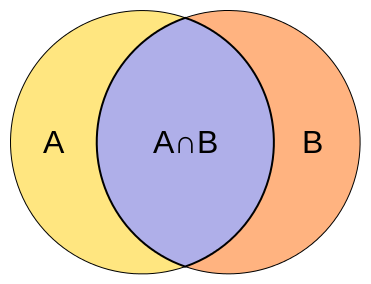
\includegraphics[width=0.75\textwidth]{images/Intersection_of_sets_A_and_B.png} 
                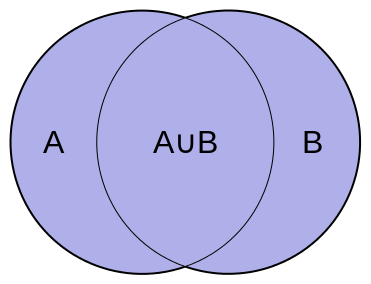
\includegraphics[width=0.75\textwidth]{images/Union_of_sets_A_and_B.png}
                \caption{Schnitt und Vereinigung zweier Mengen $ A $ und $ B $ \cite{intersectionImage,unionImage}}
            \end{figure}        
        \end{column}
    \end{columns}
\end{frame}



\section{MinHash}

\begin{frame}{MinHash I \cite{minhash}}
    \begin{itemize}
        \item Algorithmus aus der Textanalyse
        \item Wurde erstmalig verwendet um eine große Menge von Webseiten miteinader zu vergleichen
        \item Arbeitet mit k-shingles
        \item Nährt den Jaccard-Koeffizienten
    \end{itemize}
\end{frame}

\begin{frame}{MinHash I \cite{minhash}}
    Die Mengen der geshingelten werden als Sparse-Matrix $ M $ dargestellt.
    
    \begin{example}
        \begin{equation*}
            M = 
            \bbordermatrix{
                & D_1 & D_2 \\
                ATG & 1 & 0 \\
                TGG & 1 & 1 \\
                GGC & 1 & 1 \\
                GCA & 1 & 1 \\
                CAT & 1 & 0 \\
                CAG & 0 & 1 \\
                AGT & 0 & 1
            }
        \end{equation*}
    \end{example}
\end{frame}
\section{Rkmh}

\begin{frame}{Rkmh I}
    \begin{columns} % align columns
        \begin{column}{.60\textwidth}
            \begin{itemize}
                \item Hyperparameter: k-mer-size $ k $, sketch-size $ s $ \pause
                \item Reads und Referenzgenom werden zu k-mers umgewandelt \pause
                \item k-mers werden gehasht \pause
                \item Die Hashs werden sortiert und die ersten $ s $ für den Vergleich genommen \pause
                \item Weitere Reduzierung der Datenmenge durch Bereitstellung von unterschiedliche Filtern \pause
            \end{itemize}
        \end{column}
        \hfill
        \begin{column}{.40\textwidth}
            \begin{figure}[H]
                \centering
                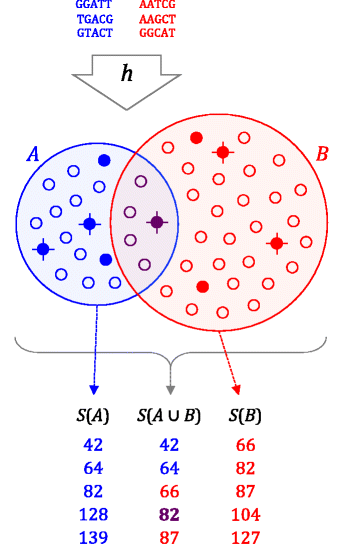
\includegraphics[width=0.85\textwidth]{images/mash_similarity.png} 
                \caption{Reduzierung der Datenmenge über MinHash \cite{mashSimilarityImage}}
            \end{figure}
        \end{column}
    \end{columns}
\end{frame}


\begin{frame}{Rkmh II}
    \begin{itemize}
        \item Beispiel-Filter\footnote{\url{https://github.com/edawson/rkmh}}: 
        \begin{itemize}
            \item --min-kmer-occurence <int>: Entfernt k-mers die nur <int> mal auftreten
            \item --max-samples <int>: Entfernt k-mers die in mehr als <int> Referenzgenomen auftreten
        \end{itemize} \pause
        \item Entwickelt in C++ mit OpenMP \pause
        \item Hash-Funktion: MurMurHash3\footnote{\url{https://github.com/aappleby/smhasher/wiki/MurmurHash3}}
    \end{itemize}
\end{frame}

\begin{frame}{Rkmh III - Ergebnisse}
    \begin{columns} % align columns
        \begin{column}{.45\textwidth}
            \begin{itemize}
                \item Umfassende Tests wurden auf verschiedenen Datensätzen sowie Testdaten\footnotemark[1] durchgeführt \pause
                \item Gute Hyperparameter-Einstellungen sketch-size  $ s \geq 4000 $ k-mer-size $ 10 < k \leq 18 $ \pause
            \end{itemize}
        \end{column}
        \begin{column}{.50\textwidth}
            \begin{figure}[H]
                \centering
                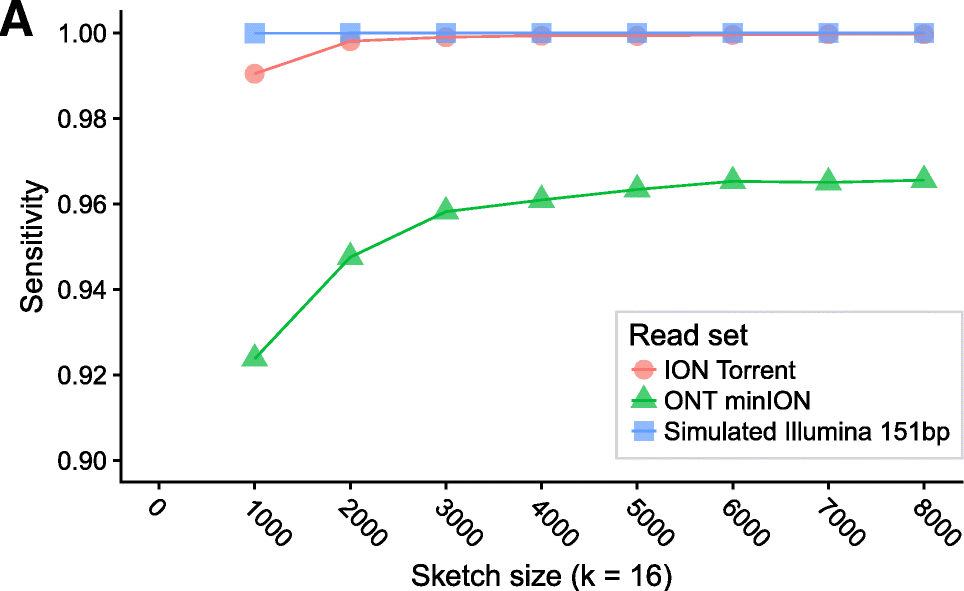
\includegraphics[width=0.85\textwidth]{images/hyper-params-a.png} 
                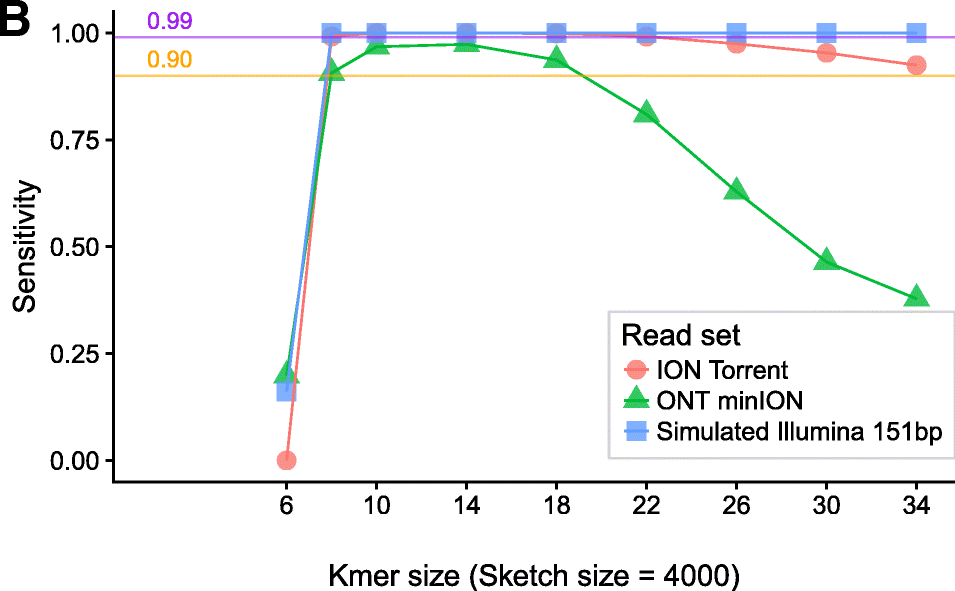
\includegraphics[width=0.85\textwidth]{images/hyper-params-b.png}
                \caption{Ermittlung von optimalem $ s $ und $ k $ \cite{rkmhHyperParamImageA,rkmhHyperParamImageB}}
            \end{figure} 
        \end{column}
    \end{columns}        

    \footnotetext[1]{\url{https://github.com/edawson/rkmh_sim_data}}
\end{frame}
\section{Fazit}

\begin{frame}{Fazit}
    \begin{itemize}
        \item Test
    \end{itemize}
\end{frame}
\begin{frame}{Vielen Dank für Ihre Aufmerksamkeit}
    \begin{center}
        Fragen?
    \end{center}
\end{frame}

\section{Quellen}

\begin{frame}[allowframebreaks]{Quellen- und Literaturverzeichnis}
    \printbibliography[heading=none, notkeyword={image}, notkeyword={online}]   
\end{frame}

% \begin{frame}[allowframebreaks]{Onlinequellen}
%     \printbibliography[heading=none, keyword={online}]    
% \end{frame}

\begin{frame}[allowframebreaks]{Bildverzeichnis}
    \printbibliography[heading=none, keyword={image}]
\end{frame}

\end{document}
